% Ensure that you compile using XeLaTeX !!! PDFTex has problems with some of the packages used
\documentclass[12pt]{article}
\setlength\parindent{0pt}

\usepackage{parskip}
\usepackage[margin=0.5in]{geometry}
\usepackage{fullpage}
\usepackage{moresize}
\usepackage{graphicx}
\usepackage{caption}
%\usepackage{subcaption}
\usepackage{float}
\usepackage{xcolor}
\usepackage{soul}
\usepackage{fontspec}
\setmainfont{Doulos SIL}

\begin{document}

\begin{center}
\textbf{{\color{violet}{\HUGE ALL QUESTIONS\\}}}

\textbf{{\color{violet}{\HUGE BY TOPIC\\}}}

\end{center}
\newpage

\textbf{\underline{\huge Other / easy\\}}

~\\

{\large Question 1} - Source: Quiz 1, Question 7\\

Is this sentence prescriptive or descriptive? Explain why.\\

People speaking standard North American English use <doesn't> with the pronoun <he>, as in ``He doesn't seem concerned today.''


~\\
INSTRUCTOR NOTES: 


~\\

{\large Question 2} - Source: Quiz 1, Question 7\\

Is this sentence prescriptive or descriptive? Explain why.\\

People who say <ain't> may suffer some negative social consequences, because many speakers of English associate <ain't> with a lack of education.


~\\
INSTRUCTOR NOTES: 


~\\

{\large Question 3} - Source: Quiz 1, Question 7\\

Is this sentence prescriptive or descriptive? Explain why.\\

In casual styles of speaking, English speakers frequently end sentences with prepositions, but ending sentences with prepositions is avoided in formal styles.


~\\
INSTRUCTOR NOTES: 


~\\

{\large Question 4} - Source: Quiz 1, Question 7\\

Is this sentence prescriptive or descriptive? Explain why.\\

Saying ``Between you and me'' is correct; saying ``Between you and I'' is ungrammatical.


~\\
INSTRUCTOR NOTES: 


~\\

{\large Question 5} - Source: Quiz 2, Question 11\\

Does the morpheme ‘eye’ occur in this word? Why or why not?\\

<Eiffel> (as in Eiffel Tower)


~\\
INSTRUCTOR NOTES: 


~\\

{\large Question 6} - Source: Quiz 2, Question 11\\

Does the morpheme ‘eye’ occur in this word? Why or why not?\\

<disobeyed>


~\\
INSTRUCTOR NOTES: 


~\\

{\large Question 7} - Source: Quiz 2, Question 11\\

Does the morpheme ‘eye’ occur in this word? Why or why not?\\

<eyeglasses>


~\\
INSTRUCTOR NOTES: 


~\\

{\large Question 8} - Source: Quiz 2, Question 11\\

Does the morpheme ‘eye’ occur in this word? Why or why not?\\

<island>


~\\
INSTRUCTOR NOTES: 


~\\

{\large Question 9} - Source: Quiz 2, Question 11\\

Does the morpheme ‘eye’ occur in this word? Why or why not?\\

<eyes>


~\\
INSTRUCTOR NOTES: 


~\\

{\large Question 10} - Source: Quiz 2, Question 11\\

Does the morpheme ‘eye’ occur in this word? Why or why not?\\

<eyeful>


~\\
INSTRUCTOR NOTES: 


~\\

{\large Question 11} - Source: Quiz 2, Question 11\\

Does the morpheme ‘eye’ occur in this word? Why or why not?\\

<spyglass>


~\\
INSTRUCTOR NOTES: 


~\\

{\large Question 12} - Source: Quiz 4, Question 1\\

Explain why the following statement is false.\\

A phoneme can be defined as the smallest unit of sound that has a meaning.


~\\
INSTRUCTOR NOTES: 


\newpage\textbf{\underline{\huge Other / medium\\}}

~\\

{\large Question 1} - Source: Day 4 Handout, Question 2(iii)\\

Explain how you would figure out the meaning of this Swahili word.\\

{[alikusumbua]}

\begin{figure}[H]
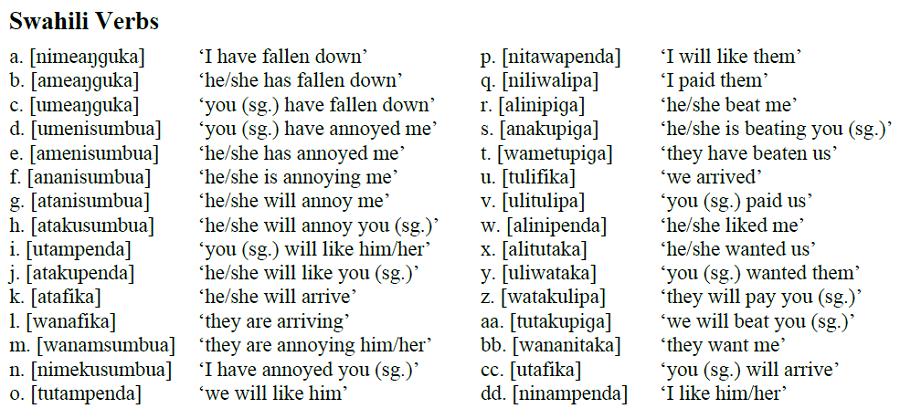
\includegraphics{../images/swahiliverbs.png}
\end{figure}

~\\
INSTRUCTOR NOTES: (he/she annoyed you (sg.))


~\\

{\large Question 2} - Source: Day 4 Handout, Question 2(iii)\\

Explain how you would figure out the meaning of this Swahili word.\\

{[tunampenda]}

\begin{figure}[H]
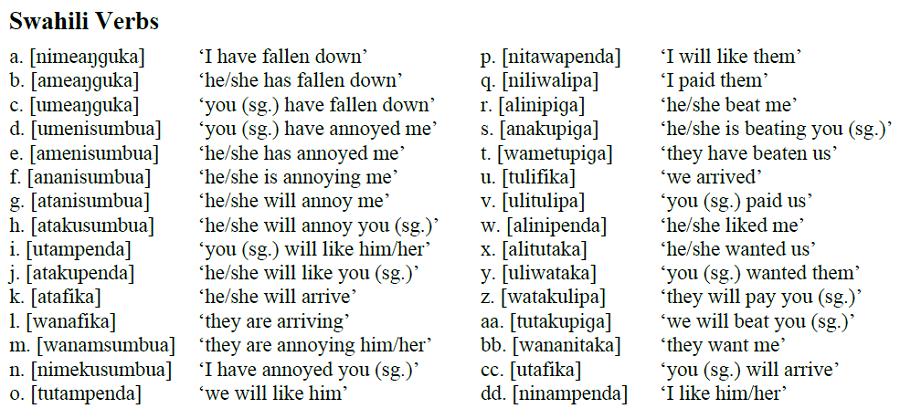
\includegraphics{../images/swahiliverbs.png}
\end{figure}

~\\
INSTRUCTOR NOTES: (we like him/her)


~\\

{\large Question 3} - Source: Day 4 Handout, Question 2(iii)\\

Explain how you would figure out the meaning of this Swahili word.\\

{[umefika]}

\begin{figure}[H]
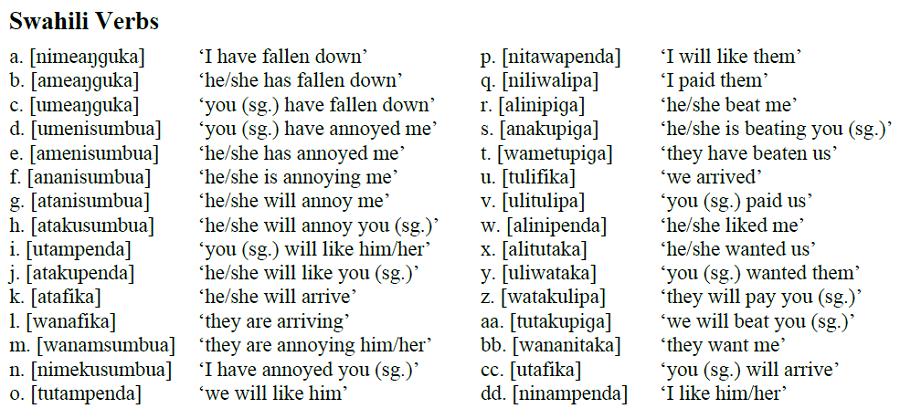
\includegraphics{../images/swahiliverbs.png}
\end{figure}

~\\
INSTRUCTOR NOTES: (you (sg.) have arrived)


~\\

{\large Question 4} - Source: Day 4 Handout, Question 2(iii)\\

Explain how you would figure out the meaning of this Swahili word.\\

{[watanipiɡa]}

\begin{figure}[H]
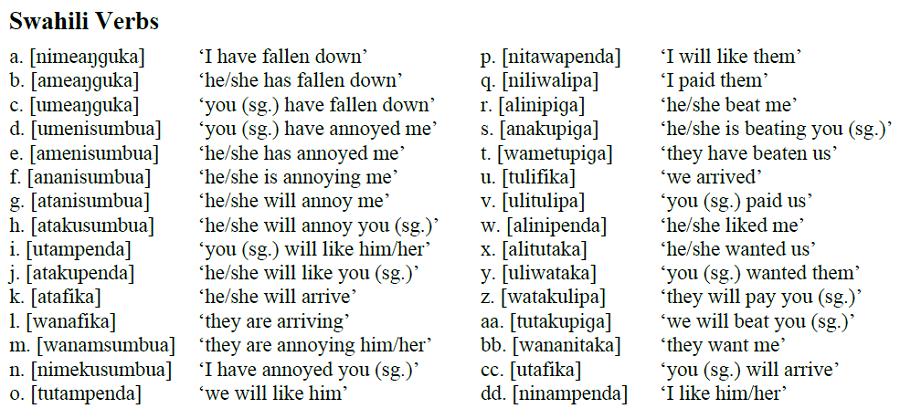
\includegraphics{../images/swahiliverbs.png}
\end{figure}

~\\
INSTRUCTOR NOTES: (they will beat me)


~\\

{\large Question 5} - Source: Day 4 Handout, Question 2(iv)\\

Explain how you would figure out the Swahili word for this English gloss.\\

‘I like you (sg.).’

\begin{figure}[H]
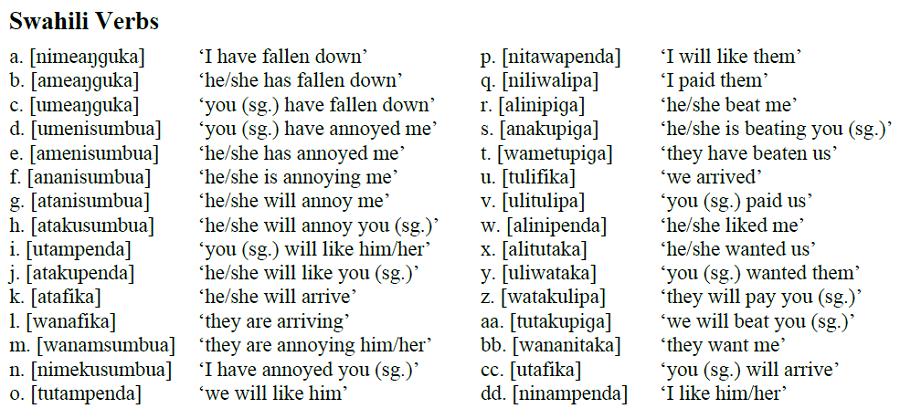
\includegraphics{../images/swahiliverbs.png}
\end{figure}

~\\
INSTRUCTOR NOTES: ([ninakupenda])


~\\

{\large Question 6} - Source: Day 4 Handout, Question 2(iv)\\

Explain how you would figure out the Swahili word for this English gloss.\\

‘We have fallen down.’

\begin{figure}[H]
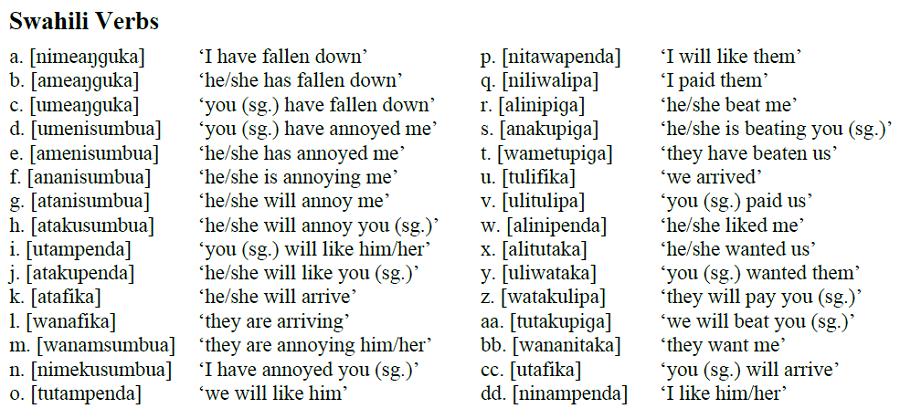
\includegraphics{../images/swahiliverbs.png}
\end{figure}

~\\
INSTRUCTOR NOTES: ([tumeaŋɡuka])


~\\

{\large Question 7} - Source: Day 4 Handout, Question 2(iv)\\

Explain how you would figure out the Swahili word for this English gloss.\\

‘She will beat us.’

\begin{figure}[H]
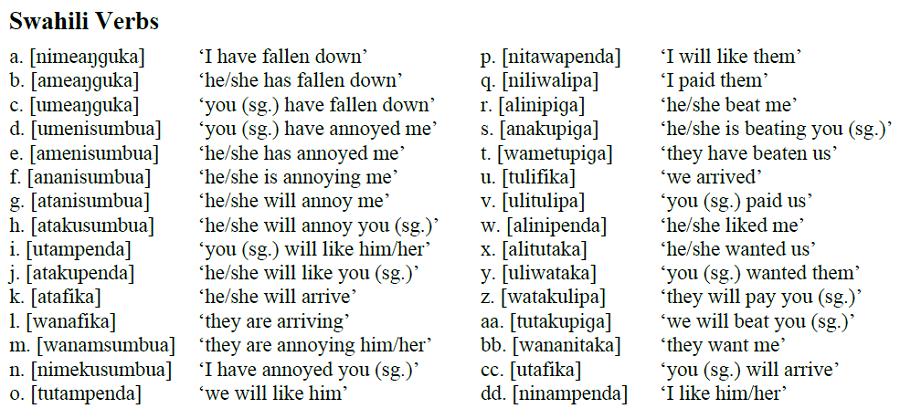
\includegraphics{../images/swahiliverbs.png}
\end{figure}

~\\
INSTRUCTOR NOTES: ([atatupiga])


~\\

{\large Question 8} - Source: Day 4 Handout, Question 2(iv)\\

Explain how you would figure out the Swahili word for this English gloss.\\

‘You (sg.) are annoying me.’

\begin{figure}[H]
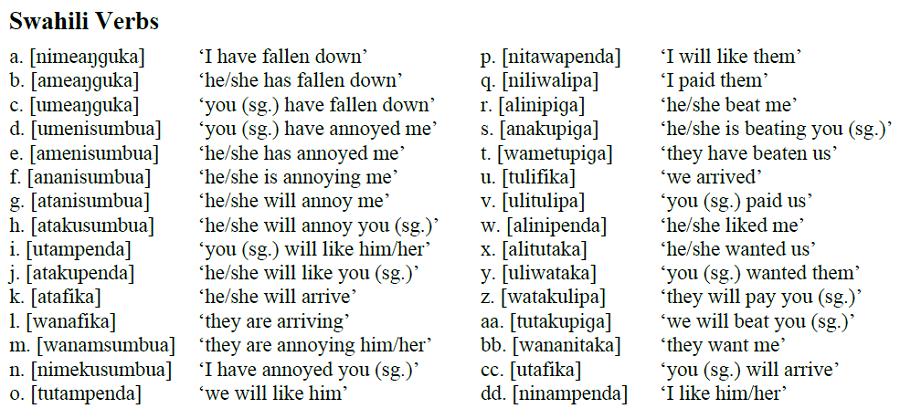
\includegraphics{../images/swahiliverbs.png}
\end{figure}

~\\
INSTRUCTOR NOTES: ([unanisumbua])


~\\

{\large Question 9} - Source: Day 4 Handout, Question 2(iv)\\

Explain how you would figure out the Swahili word for this English gloss.\\

‘They will pay him.’

\begin{figure}[H]
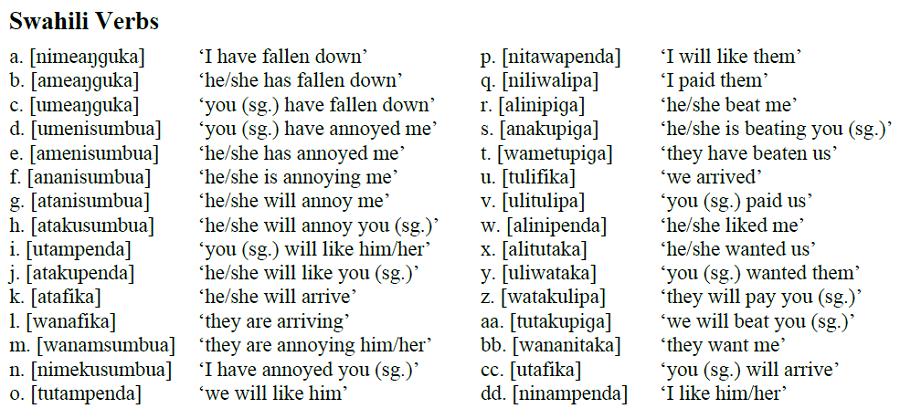
\includegraphics{../images/swahiliverbs.png}
\end{figure}

~\\
INSTRUCTOR NOTES: ([watamlipa])


~\\

{\large Question 10} - Source: Day 4 Handout, Question 2(iv)\\

Explain how you would figure out the Swahili word for this English gloss.\\

‘I wanted them.’

\begin{figure}[H]
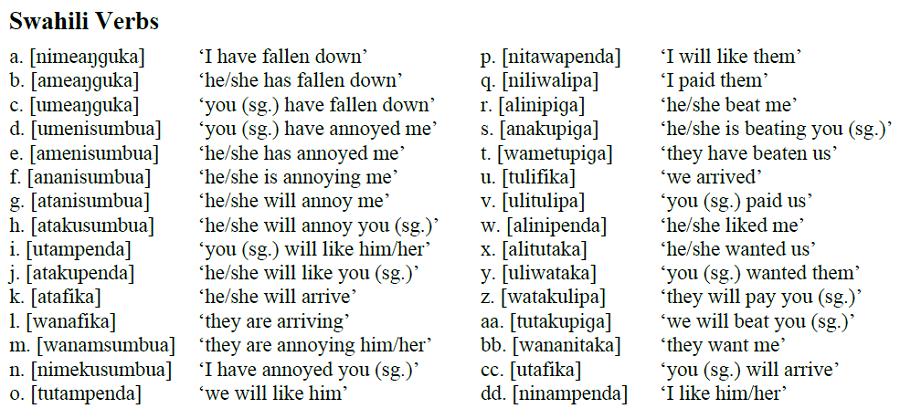
\includegraphics{../images/swahiliverbs.png}
\end{figure}

~\\
INSTRUCTOR NOTES: ([niliwataka])


~\\

{\large Question 11} - Source: Day 4 Handout, Question 3\\

Explain how you would figure out what the Luiseño form is for the morpheme whose meaning is given below.\\

‘first person singular subject’ (‘I’)

\begin{figure}[H]
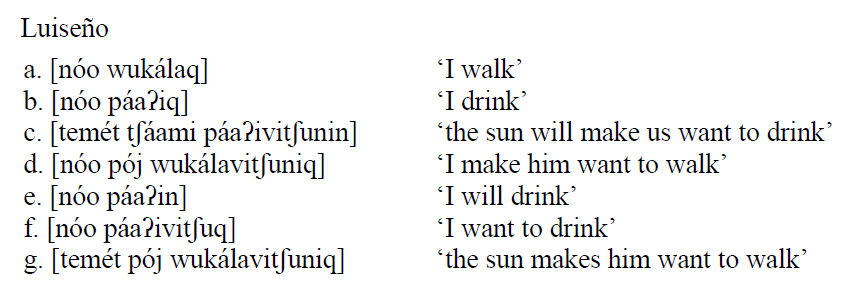
\includegraphics{../images/luiseno.png}
\end{figure}

~\\
INSTRUCTOR NOTES: ([nóo])


~\\

{\large Question 12} - Source: Day 4 Handout, Question 3\\

Explain how you would figure out what the Luiseño form is for the morpheme whose meaning is given below.\\

‘first person plural object’ (‘us’)

\begin{figure}[H]
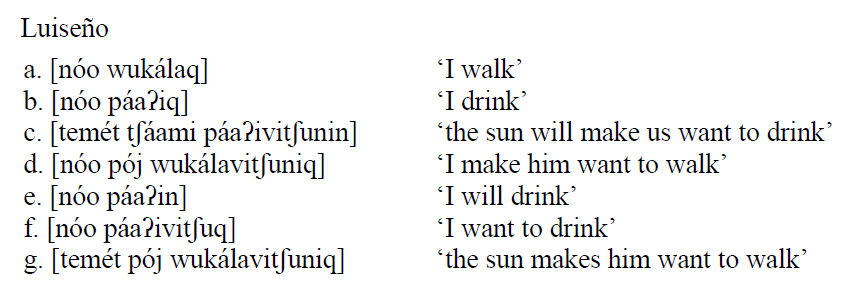
\includegraphics{../images/luiseno.png}
\end{figure}

~\\
INSTRUCTOR NOTES: ([tʃáami])


~\\

{\large Question 13} - Source: Day 4 Handout, Question 3\\

Explain how you would figure out what the Luiseño form is for the morpheme whose meaning is given below.\\

‘walk’

\begin{figure}[H]
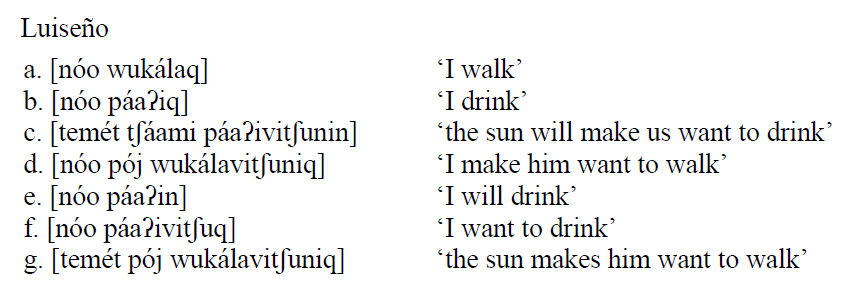
\includegraphics{../images/luiseno.png}
\end{figure}

~\\
INSTRUCTOR NOTES: ([wukála])


~\\

{\large Question 14} - Source: Day 4 Handout, Question 3\\

Explain how you would figure out what the Luiseño form is for the morpheme whose meaning is given below.\\

‘want’

\begin{figure}[H]
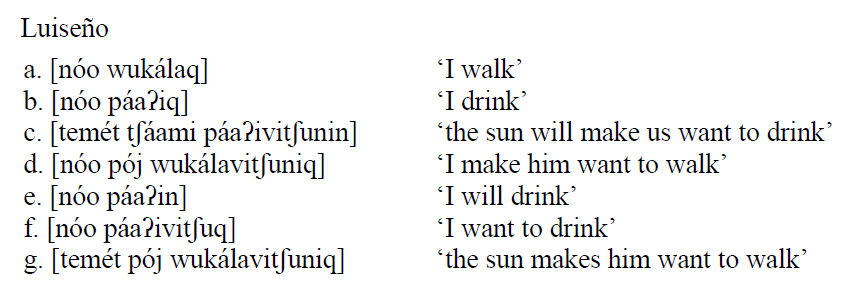
\includegraphics{../images/luiseno.png}
\end{figure}

~\\
INSTRUCTOR NOTES: ([vitʃu])


~\\

{\large Question 15} - Source: Day 4 Handout, Question 3\\

Explain how you would figure out what the Luiseño form is for the morpheme whose meaning is given below.\\

‘present tense’

\begin{figure}[H]
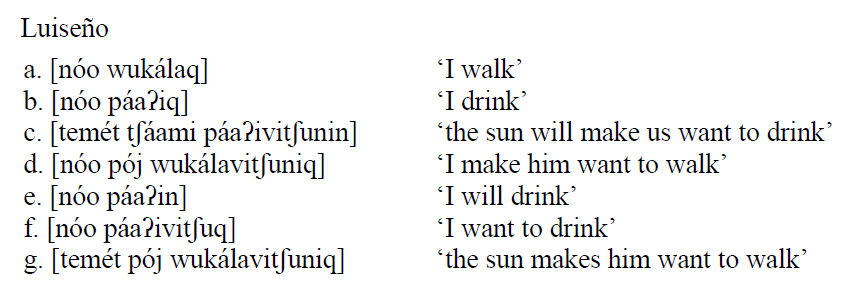
\includegraphics{../images/luiseno.png}
\end{figure}

~\\
INSTRUCTOR NOTES: ([q])


~\\

{\large Question 16} - Source: Day 4 Handout, Question 3\\

Explain how you would figure out what the Luiseño form is for the morpheme whose meaning is given below.\\

‘third person masc. object’ (‘him’)

\begin{figure}[H]
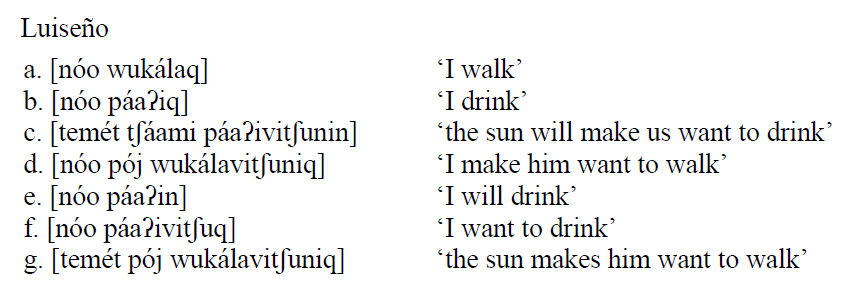
\includegraphics{../images/luiseno.png}
\end{figure}

~\\
INSTRUCTOR NOTES: ([pój])


~\\

{\large Question 17} - Source: Day 4 Handout, Question 3\\

Explain how you would figure out what the Luiseño form is for the morpheme whose meaning is given below.\\

‘sun’ (or ‘the sun’)

\begin{figure}[H]
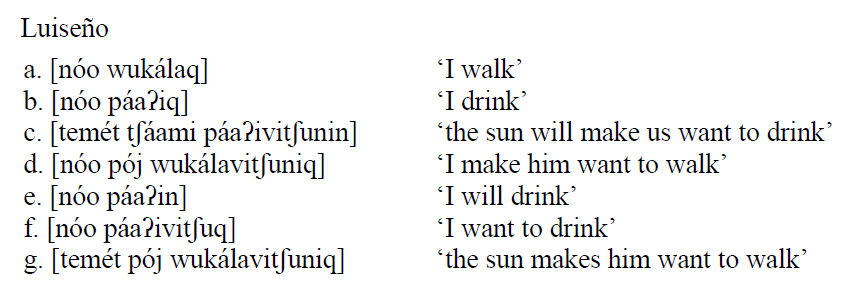
\includegraphics{../images/luiseno.png}
\end{figure}

~\\
INSTRUCTOR NOTES: ([temét])


~\\

{\large Question 18} - Source: Day 4 Handout, Question 3\\

Explain how you would figure out what the Luiseño form is for the morpheme whose meaning is given below.\\

‘drink’

\begin{figure}[H]
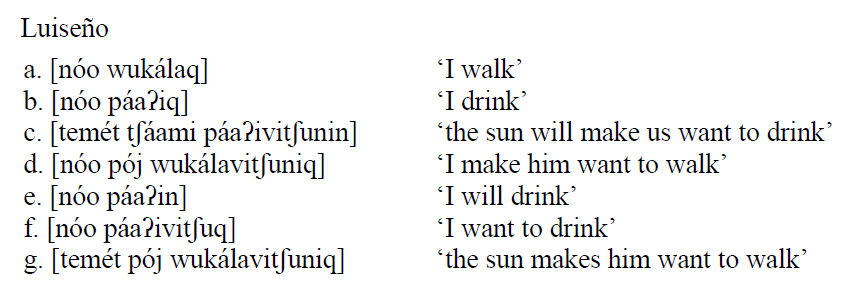
\includegraphics{../images/luiseno.png}
\end{figure}

~\\
INSTRUCTOR NOTES: ([páaʔi])


~\\

{\large Question 19} - Source: Day 4 Handout, Question 3\\

Explain how you would figure out what the Luiseño form is for the morpheme whose meaning is given below.\\

‘make / cause’

\begin{figure}[H]
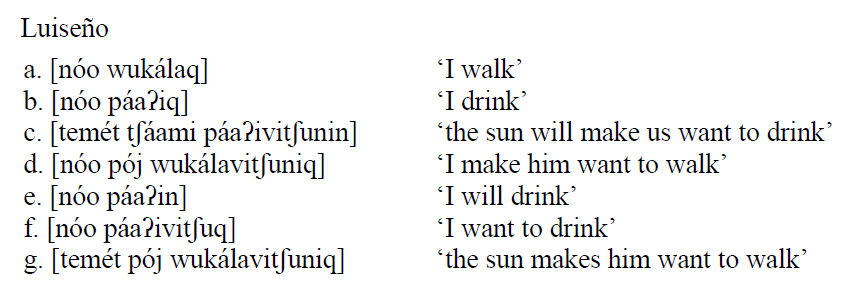
\includegraphics{../images/luiseno.png}
\end{figure}

~\\
INSTRUCTOR NOTES: ([ni])


~\\

{\large Question 20} - Source: Day 4 Handout, Question 3\\

Explain how you would figure out what the Luiseño form is for the morpheme whose meaning is given below.\\

‘Future’

\begin{figure}[H]
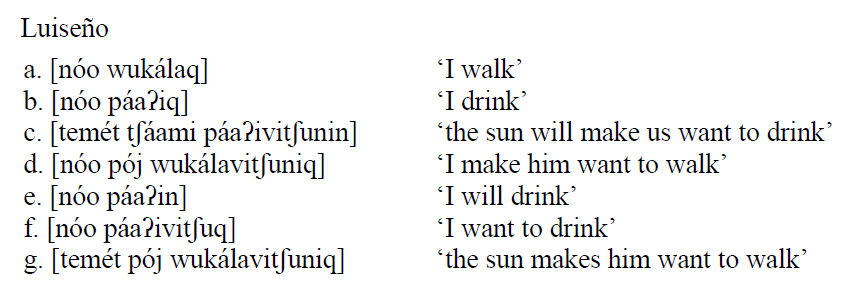
\includegraphics{../images/luiseno.png}
\end{figure}

~\\
INSTRUCTOR NOTES: ([n])


~\\

{\large Question 21} - Source: Day 4 Discussion\\

Explain what we mean by saying that linguistic patterns are \underline{productive}.\\


~\\
INSTRUCTOR NOTES: 


~\\

{\large Question 22} - Source: Homework 2, Question 1\\

What would this Klingon phrase below be in English? How do you know?\\

{[pɑdɑq]}

\begin{figure}[H]
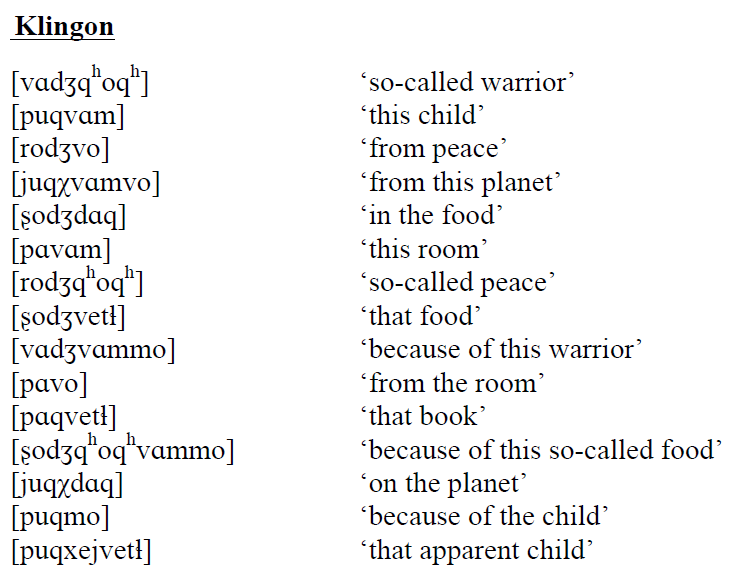
\includegraphics{../images/klingon.png}
\end{figure}

~\\
INSTRUCTOR NOTES: ‘in/on (the) room’


~\\

{\large Question 23} - Source: Homework 2, Question 1\\

What would this Klingon phrase below be in English? How do you know?\\

{[vɑdʒqʰoqʰvɑm]}

\begin{figure}[H]
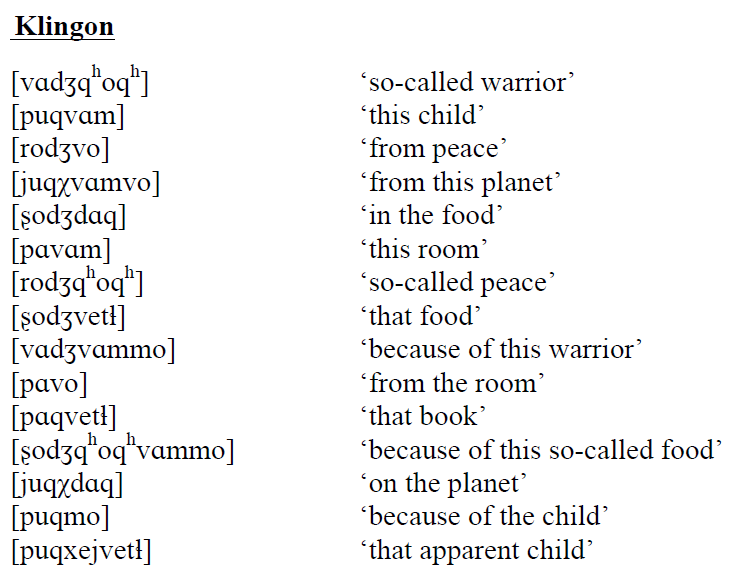
\includegraphics{../images/klingon.png}
\end{figure}

~\\
INSTRUCTOR NOTES: ‘this so-called warrior’


~\\

{\large Question 24} - Source: Homework 2, Question 1\\

What would this Klingon phrase below be in English? How do you know?\\

{[pɑqqʰoqʰvetɬvo]}

\begin{figure}[H]
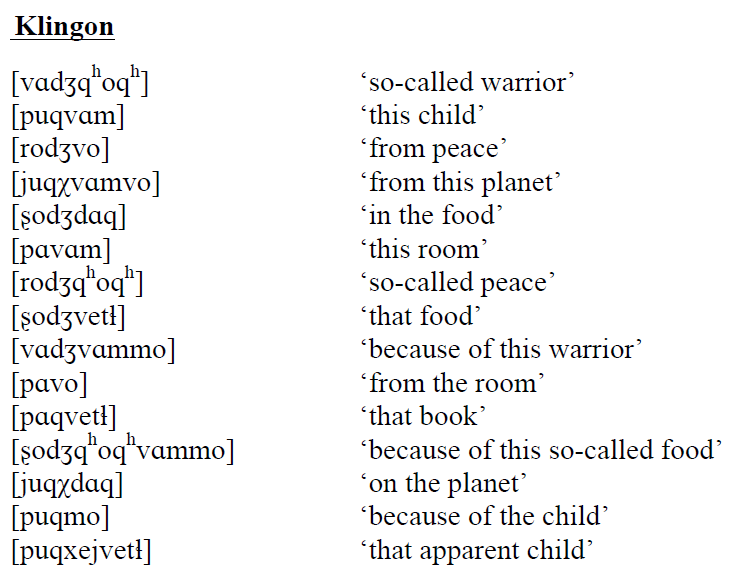
\includegraphics{../images/klingon.png}
\end{figure}

~\\
INSTRUCTOR NOTES: ‘from that so-called book’


\newpage\textbf{\underline{\huge Articulatory Phonetics / hard\\}}

~\\

{\large Question 1} - Source: Day 2 Discussion\\

Explain why it's possible to say that signed languages have articulatory phonetics.\\


~\\
INSTRUCTOR NOTES: 


~\\

{\large Question 2} - Source: Day 2 Handout, Part II, Question 5\\

Based on this data, explain how the concept of natural classes helps us be able to make predictions about whether new words in this language would start with [b] or [k].\\

\begin{itemize} \item {[bido]} \item {[benɑ]} \item {[kulɑ]} \item {[koni]} \end{itemize}


~\\
INSTRUCTOR NOTES: 


~\\

{\large Question 3} - Source: Day 2 Handout, Part II, Question 6\\

Based on this data, explain how the concept of natural classes helps us be able to make predictions about whether new words in this language would start with [b] or [k].\\

\begin{itemize} \item {[budo]} \item {[bɪne]} \item {[kilɑ]} \item {[kɑno]} \end{itemize}


~\\
INSTRUCTOR NOTES: 


~\\

{\large Question 4} - Source: Homework 1, Question 3(a)\\

Could this image be the result of producing the sound represented by the given IPA symbol? Why or why not?\\

{[d]}

\begin{figure}[H]
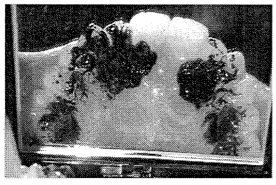
\includegraphics{../images/staticpalatography_fricative.png}
\end{figure}

~\\
INSTRUCTOR NOTES: no; space


~\\

{\large Question 5} - Source: Homework 1, Question 3(a)\\

Could this image be the result of producing the sound represented by the given IPA symbol? Why or why not?\\

{[z]}

\begin{figure}[H]
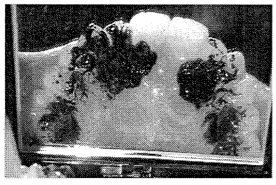
\includegraphics{../images/staticpalatography_fricative.png}
\end{figure}

~\\
INSTRUCTOR NOTES: yes


~\\

{\large Question 6} - Source: Homework 1, Question 3(a)\\

Could this image be the result of producing the sound represented by the given IPA symbol? Why or why not?\\

{[n]}

\begin{figure}[H]
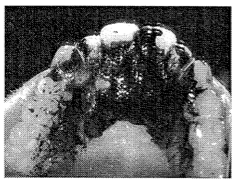
\includegraphics{../images/staticpalatography_stop.png}
\end{figure}

~\\
INSTRUCTOR NOTES: yes


~\\

{\large Question 7} - Source: Homework 1, Question 3(a)\\

Could this image be the result of producing the sound represented by the given IPA symbol? Why or why not?\\

{[t͡ʃ]}

\begin{figure}[H]
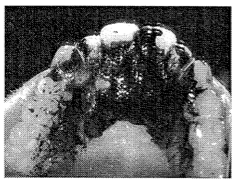
\includegraphics{../images/staticpalatography_stop.png}
\end{figure}

~\\
INSTRUCTOR NOTES: yes


~\\

{\large Question 8} - Source: Homework 1, Question 3(a)\\

Could this image be the result of producing the sound represented by the given IPA symbol? Why or why not?\\

{[t͡ʃ]}

\begin{figure}[H]
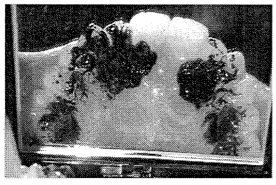
\includegraphics{../images/staticpalatography_fricative.png}
\end{figure}

~\\
INSTRUCTOR NOTES: no


~\\

{\large Question 9} - Source: Homework 1, Question 3(a)\\

Could this image be the result of producing the sound represented by the given IPA symbol? Why or why not?\\

{[ɾ]}

\begin{figure}[H]
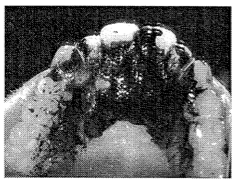
\includegraphics{../images/staticpalatography_stop.png}
\end{figure}

~\\
INSTRUCTOR NOTES: yes


\newpage\textbf{\underline{\huge Articulatory Phonetics / medium\\}}

~\\

{\large Question 1} - Source: Day 2 Discussion\\

Assuming a Standard North American English inventory, does this vowel need to have tenseness specified if you're giving a prose description? Why or why not?\\

{[æ]}


~\\
INSTRUCTOR NOTES: no


~\\

{\large Question 2} - Source: Day 2 Discussion\\

Assuming a Standard North American English inventory, does this vowel need to have tenseness specified if you're giving a prose description? Why or why not?\\

{[ɑ]}


~\\
INSTRUCTOR NOTES: no


~\\

{\large Question 3} - Source: Day 2 Discussion\\

Assuming a Standard North American English inventory, does this vowel need to have tenseness specified if you're giving a prose description? Why or why not?\\

{[i]}


~\\
INSTRUCTOR NOTES: yes


~\\

{\large Question 4} - Source: Day 2 Discussion\\

Assuming a Standard North American English inventory, does this vowel need to have tenseness specified if you're giving a prose description? Why or why not?\\

{[u]}


~\\
INSTRUCTOR NOTES: yes


~\\

{\large Question 5} - Source: Day 2 Discussion\\

Assuming a Standard North American English inventory, does this vowel need to have tenseness specified if you're giving a prose description? Why or why not?\\

{[ɛ]}


~\\
INSTRUCTOR NOTES: yes


~\\

{\large Question 6} - Source: Day 2 Discussion\\

Assuming a Standard North American English inventory, does this vowel need to have tenseness specified if you're giving a prose description? Why or why not?\\

{[ɔ]}


~\\
INSTRUCTOR NOTES: yes


~\\

{\large Question 7} - Source: Quiz 2, Question 6\\

In the pronunciation of this word, which sounds are obstruents and which are sonorants?\\

<sonorant>


~\\
INSTRUCTOR NOTES: [sɔnoɹənt] -- sonorants: [ɔnoɹən] and obstruents: [st]


~\\

{\large Question 8} - Source: Quiz 2, Question 6\\

In the pronunciation of this word, which sounds are obstruents and which are sonorants?\\

<obstruent>


~\\
INSTRUCTOR NOTES: [ɑbstɹuənt] -- sonorants: [ɑɹuən] and obstruents: [bstt]


~\\

{\large Question 9} - Source: Quiz 2, Question 6\\

In the pronunciation of this word, which sounds are obstruents and which are sonorants?\\

<minimal>


~\\
INSTRUCTOR NOTES: [mɪnɪməl] -- sonorants: (all of them)


~\\

{\large Question 10} - Source: Quiz 2, Question 6\\

In the pronunciation of this word, which sounds are obstruents and which are sonorants?\\

<language>


~\\
INSTRUCTOR NOTES: [læŋɡwɪdʒ] -- sonorants: [læŋwɪ] and obstruents: [ɡdʒ]


~\\

{\large Question 11} - Source: Quiz 2, Question 6\\

In the pronunciation of this word, which sounds are obstruents and which are sonorants?\\

<fricative>


~\\
INSTRUCTOR NOTES: [fɹɪkətɪv] -- sonorants: [ɹɪəɪ] and obstruents: [fktv]


~\\

{\large Question 12} - Source: Quiz 2, Question 7\\

Why might two of the descriptions given truthfully apply to the sound represented by the underlined letter, and why is one of them actually better than the other?\\

<a\underline{w}ay>

\begin{itemize} \item prevocalic obstruent \item prevocalic sonorant \item postvocalic obstruent \item postvocalic sonorant \item intervocalic obstruent \item intervocalic sonorant \end{itemize}


~\\
INSTRUCTOR NOTES: prevocalic and *intervocalic* sonorant


~\\

{\large Question 13} - Source: Day 2 Handout, Part II, Question 7\\

Is the symbol given a reasonable way to transcribe any of the sounds described below? If so, which one? If not, why not?\\

{[n]}

\begin{itemize} \item voiceless palatal affricate \item voiced velar nasal \item voiceless glottal fricative \item voiced labiodental fricative \item voiced interdental fricative \item voiced palatal fricative \end{itemize}


~\\
INSTRUCTOR NOTES: no (voiced alveolar nasal)


~\\

{\large Question 14} - Source: Day 2 Handout, Part II, Question 7\\

Is the symbol given a reasonable way to transcribe any of the sounds described below? If so, which one? If not, why not?\\

{[h]}

\begin{itemize} \item voiceless palatal affricate \item voiced velar nasal \item voiceless glottal fricative \item voiced labiodental fricative \item voiced interdental fricative \item voiced palatal fricative \end{itemize}


~\\
INSTRUCTOR NOTES: yes (voiceless glottal fricative)


~\\

{\large Question 15} - Source: Day 2 Handout, Part II, Question 7\\

Is the symbol given a reasonable way to transcribe any of the sounds described below? If so, which one? If not, why not?\\

{[v]}

\begin{itemize} \item voiceless palatal affricate \item voiced velar nasal \item voiceless glottal fricative \item voiced labiodental fricative \item voiced interdental fricative \item voiced palatal fricative \end{itemize}


~\\
INSTRUCTOR NOTES: yes (voiced labiodental fricative)


~\\

{\large Question 16} - Source: Day 2 Handout, Part II, Question 7\\

Is the symbol given a reasonable way to transcribe any of the sounds described below? If so, which one? If not, why not?\\

{[θ]}

\begin{itemize} \item voiceless palatal affricate \item voiced velar nasal \item voiceless glottal fricative \item voiced labiodental fricative \item voiced interdental fricative \item voiced palatal fricative \end{itemize}


~\\
INSTRUCTOR NOTES: no (voiceless interdental fricative)


~\\

{\large Question 17} - Source: Day 2 Handout, Part II, Question 7\\

Is the symbol given a reasonable way to transcribe any of the sounds described below? If so, which one? If not, why not?\\

{[ʃ]}

\begin{itemize} \item voiceless palatal affricate \item voiced velar nasal \item voiceless glottal fricative \item voiced labiodental fricative \item voiced interdental fricative \item voiced palatal fricative \end{itemize}


~\\
INSTRUCTOR NOTES: no (voiceless palatal fricative)


~\\

{\large Question 18} - Source: Day 2 Handout, Part II, Question 7\\

Is the symbol given a reasonable way to transcribe any of the sounds described below? If so, which one? If not, why not?\\

{[ʒ]}

\begin{itemize} \item voiceless palatal affricate \item voiced velar nasal \item voiceless glottal fricative \item voiced labiodental fricative \item voiced interdental fricative \item voiced palatal fricative \end{itemize}


~\\
INSTRUCTOR NOTES: yes (voiced palatal fricative)


~\\

{\large Question 19} - Source: Day 2 Handout, Part II, Question 7\\

Is the symbol given a reasonable way to transcribe any of the sounds described below? If so, which one? If not, why not?\\

{[t͡ʃ]}

\begin{itemize} \item voiceless palatal affricate \item voiced velar nasal \item voiceless glottal fricative \item voiced labiodental fricative \item voiced interdental fricative \item voiced palatal fricative \end{itemize}


~\\
INSTRUCTOR NOTES: yes (voiceless palatal affricate)


~\\

{\large Question 20} - Source: Day 2 Handout, Part II, Question 9\\

Explain how to figure out what the sound being produced is in this diagram.\\

\begin{figure}[H]
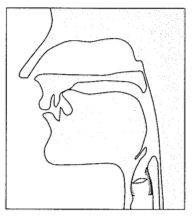
\includegraphics{../images/sagittal_t.png}
\end{figure}

~\\
INSTRUCTOR NOTES: [t] (check voicing, place, manner, and velum)


~\\

{\large Question 21} - Source: Day 2 Handout, Part II, Question 9\\

Explain how to figure out what the sound being produced is in this diagram.\\

\begin{figure}[H]
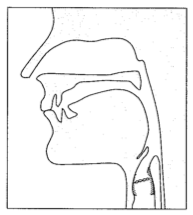
\includegraphics{../images/sagittal_m.png}
\end{figure}

~\\
INSTRUCTOR NOTES: [m] (check voicing, place, manner, and velum)


~\\

{\large Question 22} - Source: Day 2 Handout, Part II, Question 9\\

Explain how to figure out what the sound being produced is in this diagram.\\

\begin{figure}[H]
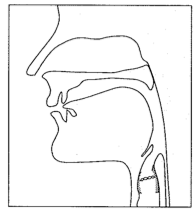
\includegraphics{../images/sagittal_eth.png}
\end{figure}

~\\
INSTRUCTOR NOTES: [ð] (check voicing, place, manner, and velum)


~\\

{\large Question 23} - Source: Day 2 Handout, Part II, Question 9\\

Explain how to figure out what the sound being produced is in this diagram.\\

\begin{figure}[H]
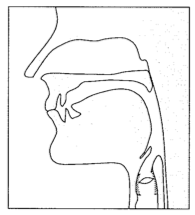
\includegraphics{../images/sagittal_p.png}
\end{figure}

~\\
INSTRUCTOR NOTES: [p] (check voicing, place, manner, and velum)


~\\

{\large Question 24} - Source: Day 2 Handout, Part II, Question 9\\

Explain how to figure out what the sound being produced is in this diagram.\\

\begin{figure}[H]
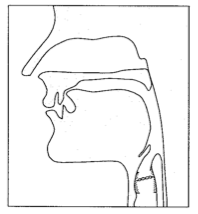
\includegraphics{../images/sagittal_z.png}
\end{figure}

~\\
INSTRUCTOR NOTES: [z] (check voicing, place, manner, and velum)


~\\

{\large Question 25} - Source: Day 2 Handout, Part II, Question 13\\

Explain why this image does or does not match the description.\\

\begin{itemize} \item A two-handed sign. \item Location: In front of signer’s chin. \item Handshape: Starts with an “L” shape; index finger and thumb come together during the sign. \item Movement: Hands start crossed and then move away from each other horizontally. \end{itemize}

\begin{figure}[H]
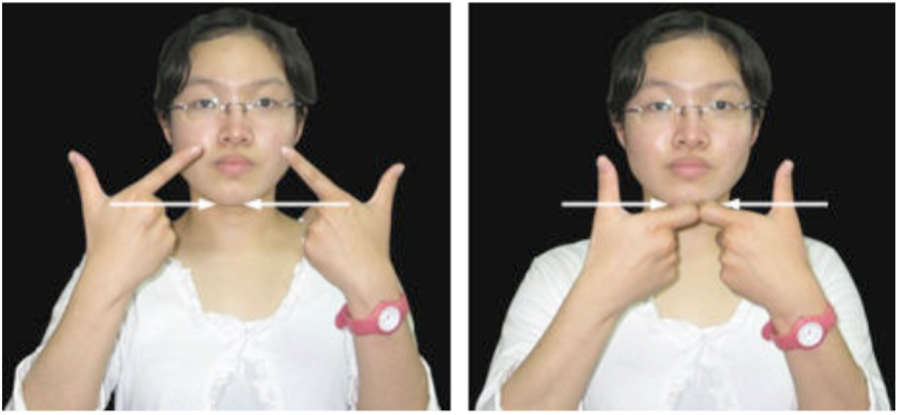
\includegraphics{../images/taiwansign_fit.png}
\caption{FIT}
\end{figure}

~\\
INSTRUCTOR NOTES: no; hands don't start crossed, and handshape change is wrong


~\\

{\large Question 26} - Source: Day 2 Handout, Part II, Question 13\\

Explain why this image does or does not match the description.\\

\begin{itemize} \item A two-handed sign. \item Location: In front of signer’s chin. \item Handshape: Starts with an “L” shape; distal joints of index fingers fold in during the sign. \item Movement: Hands start apart and then move straight toward each other horizontally. \end{itemize}

\begin{figure}[H]
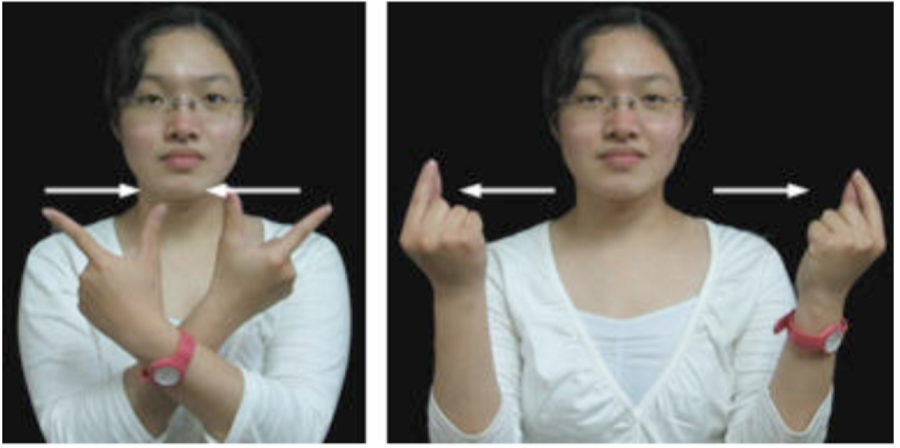
\includegraphics{../images/taiwansign_consistent.png}
\caption{CONSISTENT}
\end{figure}

~\\
INSTRUCTOR NOTES: no; hands don't start apart, and handshape change is wrong


~\\

{\large Question 27} - Source: Day 2 Handout, Part II, Question 13\\

Explain why this image does or does not match the description.\\

\begin{itemize} \item A one-handed sign. \item Location: At the signer’s nose. \item Handshape: Starts with index finger extended; finger folds down into a “hook” shape during the sign; then straightens and repeats the folding. \item Movement: No movement other than the change in handshape. \end{itemize}

\begin{figure}[H]

\includegraphics{../images/taiwansign_wrong.png}
\caption{WRONG}
\end{figure}

~\\
INSTRUCTOR NOTES: no; handshape is wrong


~\\

{\large Question 28} - Source: Day 2 Handout, Part II, Question 13\\

Explain why this image does or does not match the description.\\

\begin{itemize} \item A one-handed sign. \item Location: In front of signer’s chin. \item Handshape: Starts with an “L” shape; proximal joint of index finger folds down during the sign. \item Movement: Hand starts on far side of signer’s body and moves horizontally straight across. \end{itemize}

\begin{figure}[H]
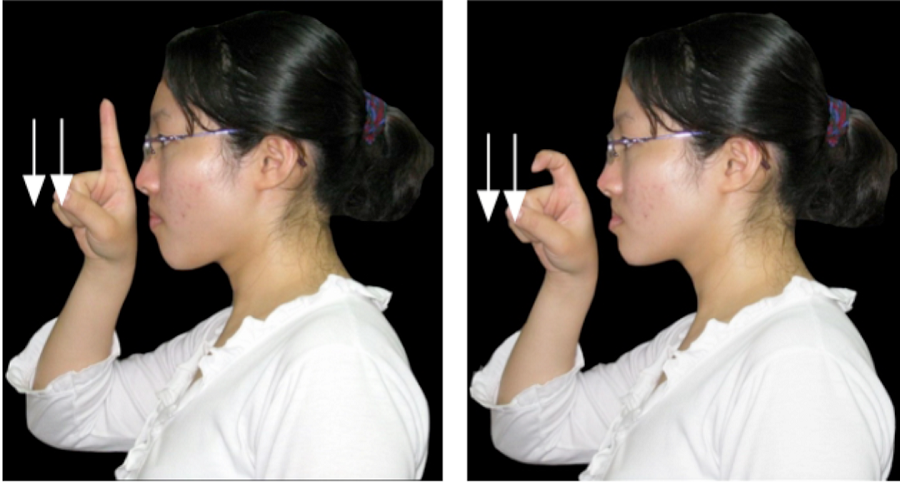
\includegraphics{../images/taiwansign_jealous.png}
\caption{JEALOUS}
\end{figure}

~\\
INSTRUCTOR NOTES: no; handshape and movement are wrong


~\\

{\large Question 29} - Source: Day 2 Handout, Part II, Question 13\\

Explain why this image does or does not match the description.\\

\begin{itemize} \item A one-handed sign. \item Location: At the signer’s nose. \item Handshape: Starts with index and middle finger crossed; the two fingers separate during the sign. \item Movement: No movement other than the change in handshape. \end{itemize}

\begin{figure}[H]
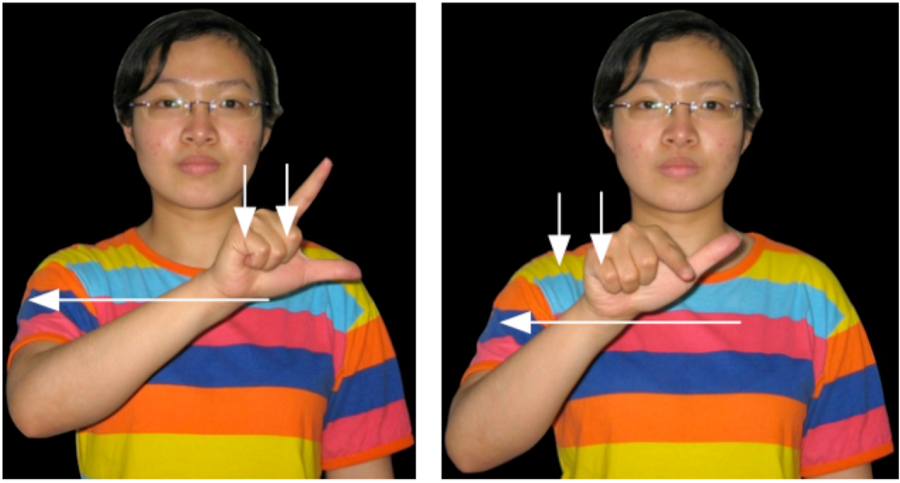
\includegraphics{../images/taiwansign_thing.png}
\caption{THING}
\end{figure}

~\\
INSTRUCTOR NOTES: no; location, movement, and handshape are all wrong


~\\

{\large Question 30} - Source: Homework 1, Question 3(b)\\

Explain why this is or is not a complete natural class in standard North American English.\\

{[p]}, {[b]}


~\\
INSTRUCTOR NOTES: yes for bilabial plosives; (no) for bilabial stops (nasal?)


~\\

{\large Question 31} - Source: Homework 1, Question 3(b)\\

Explain why this is or is not a complete natural class in standard North American English.\\

{[f]}, {[s]}, {[ʃ]}


~\\
INSTRUCTOR NOTES: no; voiceless fricatives include [θ], [h]


~\\

{\large Question 32} - Source: Homework 1, Question 3(b)\\

Explain why this is or is not a complete natural class in standard North American English.\\

{[b]}, {[n]}, {[ɡ]}, {[ʒ]}, {[v]}


~\\
INSTRUCTOR NOTES: no; lots of other voiced consonants


~\\

{\large Question 33} - Source: Homework 1, Question 3(b)\\

Explain why this is or is not a complete natural class in standard North American English.\\

{[f]}, {[θ]}, {[z]}, {[h]}


~\\
INSTRUCTOR NOTES: no; several fricatives missing


~\\

{\large Question 34} - Source: Homework 1, Question 3(b)\\

Explain why this is or is not a complete natural class in standard North American English.\\

{[j]}, {[w]}


~\\
INSTRUCTOR NOTES: yes for voiced glides; [w̥] missing for glides


~\\

{\large Question 35} - Source: Homework 1, Question 3(b)\\

Explain why this is or is not a complete natural class in standard North American English.\\

{[ɑ]}, {[u]}


~\\
INSTRUCTOR NOTES: no; several back vowels / back monophthongs missing


~\\

{\large Question 36} - Source: Homework 1, Question 3(b)\\

Explain why this is or is not a complete natural class in standard North American English.\\

{[ɔ]}, {[ʊ]}, {[u]}, {[oʊ]}


~\\
INSTRUCTOR NOTES: yes (all back rounded vowels)


~\\

{\large Question 37} - Source: Homework 1, Question 3(b)\\

Explain why this is or is not a complete natural class in standard North American English.\\

{[i]}, {[u]}, {[eɪ]}


~\\
INSTRUCTOR NOTES: no; [oʊ] missing for tense vowels


\newpage\textbf{\underline{\huge Transcription / easy\\}}

~\\

{\large Question 1} - Source: Day 2 Handout, Part I, Question 2\\

Explain why people might legitimately disagree about how many sounds this particular word contains.\\

<how>


~\\
INSTRUCTOR NOTES: 


~\\

{\large Question 2} - Source: Day 2 Handout, Part I, Question 2\\

Explain why people might legitimately disagree about how many sounds this particular word contains.\\

<tiny>


~\\
INSTRUCTOR NOTES: 


~\\

{\large Question 3} - Source: Day 2 Handout, Part I, Question 2\\

Explain why people might legitimately disagree about how many sounds this particular word contains.\\

<goat>


~\\
INSTRUCTOR NOTES: 


~\\

{\large Question 4} - Source: Day 2 Handout, Part I, Question 2\\

Explain why people might legitimately disagree about how many sounds this particular word contains.\\

<those>


~\\
INSTRUCTOR NOTES: 


~\\

{\large Question 5} - Source: Day 2 Handout, Part I, Question 2\\

Explain why people might legitimately disagree about how many sounds this particular word contains.\\

<flowers>


~\\
INSTRUCTOR NOTES: 


~\\

{\large Question 6} - Source: Day 2 Handout, Part I, Question 2\\

Explain why people might legitimately disagree about how many sounds this particular word contains.\\

<girls>


~\\
INSTRUCTOR NOTES: 


~\\

{\large Question 7} - Source: Day 2 Handout, Part I, Question 2\\

Explain why people might legitimately disagree about how many sounds this particular word contains.\\

<find>


~\\
INSTRUCTOR NOTES: 


~\\

{\large Question 8} - Source: Day 2 Handout, Part I, Question 2\\

Explain why people might legitimately disagree about how many sounds this particular word contains.\\

<they>


~\\
INSTRUCTOR NOTES: 


~\\

{\large Question 9} - Source: Day 2 Handout, Part I, Question 3\\

Explain why people might legitimately disagree about how many sounds this particular word contains.\\

<soap>


~\\
INSTRUCTOR NOTES: 


~\\

{\large Question 10} - Source: Day 2 Handout, Part I, Question 3\\

Explain why people might legitimately disagree about how many sounds this particular word contains.\\

<curtain>


~\\
INSTRUCTOR NOTES: 


~\\

{\large Question 11} - Source: Day 2 Handout, Part I, Question 3\\

Explain why people might legitimately disagree about how many sounds this particular word contains.\\

<better>


~\\
INSTRUCTOR NOTES: 


~\\

{\large Question 12} - Source: Day 2 Handout, Part I, Question 3\\

Explain why people might legitimately disagree about how many sounds this particular word contains.\\

<worse>


~\\
INSTRUCTOR NOTES: 


~\\

{\large Question 13} - Source: Day 2 Handout, Part I, Question 3\\

Explain why people might legitimately disagree about how many sounds this particular word contains.\\

<burger>


~\\
INSTRUCTOR NOTES: 


~\\

{\large Question 14} - Source: Day 2 Handout, Part I, Question 3\\

Explain why people might legitimately disagree about how many sounds this particular word contains.\\

<rice>


~\\
INSTRUCTOR NOTES: 


\newpage\textbf{\underline{\huge Transcription / medium\\}}

~\\

{\large Question 1} - Source: Day 2 Handout, Part I, Question 11\\

How would this word be transcribed?\\ Follow-up question: Why did you use symbol [X] instead of symbol [Y]?\\

<nice>


~\\
INSTRUCTOR NOTES: [nɑɪs]


~\\

{\large Question 2} - Source: Day 2 Handout, Part I, Question 11\\

How would this word be transcribed?\\ Follow-up question: Why did you use symbol [X] instead of symbol [Y]?\\

<frog>


~\\
INSTRUCTOR NOTES: [fɹɑɡ]


~\\

{\large Question 3} - Source: Day 2 Handout, Part I, Question 11\\

How would this word be transcribed?\\ Follow-up question: Why did you use symbol [X] instead of symbol [Y]?\\

<cough>


~\\
INSTRUCTOR NOTES: [kɑf]


~\\

{\large Question 4} - Source: Day 2 Handout, Part I, Question 11\\

How would this word be transcribed?\\ Follow-up question: Why did you use symbol [X] instead of symbol [Y]?\\

<juice>


~\\
INSTRUCTOR NOTES: [dʒus]


~\\

{\large Question 5} - Source: Day 2 Handout, Part I, Question 11\\

How would this word be transcribed?\\ Follow-up question: Why did you use symbol [X] instead of symbol [Y]?\\

<wealth>


~\\
INSTRUCTOR NOTES: [wɛlθ]


~\\

{\large Question 6} - Source: Day 2 Handout, Part I, Question 11\\

How would this word be transcribed?\\ Follow-up question: Why did you use symbol [X] instead of symbol [Y]?\\

<toy>


~\\
INSTRUCTOR NOTES: [tɔɪ]


~\\

{\large Question 7} - Source: Day 2 Handout, Part I, Question 11\\

How would this word be transcribed?\\ Follow-up question: Why did you use symbol [X] instead of symbol [Y]?\\

<finger>


~\\
INSTRUCTOR NOTES: [fɪŋɡɹ̩]


~\\

{\large Question 8} - Source: Day 2 Handout, Part I, Question 11\\

How would this word be transcribed?\\ Follow-up question: Why did you use symbol [X] instead of symbol [Y]?\\

<little>


~\\
INSTRUCTOR NOTES: [lɪɾl̩]


~\\

{\large Question 9} - Source: Day 2 Handout, Part I, Question 11\\

How would this word be transcribed?\\ Follow-up question: Why did you use symbol [X] instead of symbol [Y]?\\

<vacuum>


~\\
INSTRUCTOR NOTES: [vækjum]


~\\

{\large Question 10} - Source: Day 2 Handout, Part I, Question 11\\

How would this word be transcribed?\\ Follow-up question: Why did you use symbol [X] instead of symbol [Y]?\\

<bird>


~\\
INSTRUCTOR NOTES: [bɹ̩d]


~\\

{\large Question 11} - Source: Day 2 Handout, Part I, Question 11\\

How would this word be transcribed?\\ Follow-up question: Why did you use symbol [X] instead of symbol [Y]?\\

<segment>


~\\
INSTRUCTOR NOTES: [sɛɡmɛnt]


~\\

{\large Question 12} - Source: Day 2 Handout, Part I, Question 11\\

How would this word be transcribed?\\ Follow-up question: Why did you use symbol [X] instead of symbol [Y]?\\

<square>


~\\
INSTRUCTOR NOTES: [skweɪɹ]


~\\

{\large Question 13} - Source: Day 2 Handout, Part I, Question 11\\

How would this word be transcribed?\\ Follow-up question: Why did you use symbol [X] instead of symbol [Y]?\\

<goat>


~\\
INSTRUCTOR NOTES: [ɡoʊt]


\newpage\textbf{\underline{\huge Transcription / hard\\}}

~\\

{\large Question 1} - Source: Day 2 Handout\\

Is this a reasonable transcription of this word? Explain why.\\

<mouse>: {[mɔɪs]}


~\\
INSTRUCTOR NOTES: no, [ɑʊ]


~\\

{\large Question 2} - Source: Day 2 Handout\\

Is this a reasonable transcription of this word? Explain why.\\

<loud>: {[lɑud]}


~\\
INSTRUCTOR NOTES: okay, but [ɑʊ]


~\\

{\large Question 3} - Source: Day 2 Handout\\

Is this a reasonable transcription of this word? Explain why.\\

<philosophy>: {[fəlɑsəfi]}


~\\
INSTRUCTOR NOTES: yes


~\\

{\large Question 4} - Source: Day 2 Handout\\

Is this a reasonable transcription of this word? Explain why.\\

<choose>: {[t͡ʃuz]}


~\\
INSTRUCTOR NOTES: yes


~\\

{\large Question 5} - Source: Day 2 Handout\\

Is this a reasonable transcription of this word? Explain why.\\

<wimp>: {[wimp]}


~\\
INSTRUCTOR NOTES: no, [ɪ]


~\\

{\large Question 6} - Source: Day 2 Handout\\

Is this a reasonable transcription of this word? Explain why.\\

<paid>: {[peid]}


~\\
INSTRUCTOR NOTES: okay, but [eɪ]


~\\

{\large Question 7} - Source: Day 2 Handout\\

Is this a reasonable transcription of this word? Explain why.\\

<climb>: {[klɑɪm]}


~\\
INSTRUCTOR NOTES: yes


~\\

{\large Question 8} - Source: Day 2 Handout\\

Is this a reasonable transcription of this word? Explain why.\\

<shows>: {[ʃoʊs]}


~\\
INSTRUCTOR NOTES: no, [z]


~\\

{\large Question 9} - Source: Day 2 Handout\\

Is this a reasonable transcription of this word? Explain why.\\

<mine>: {[mɑɪn]}


~\\
INSTRUCTOR NOTES: yes


~\\

{\large Question 10} - Source: Day 2 Handout\\

Is this a reasonable transcription of this word? Explain why.\\

<health>: {[hɛlð]}


~\\
INSTRUCTOR NOTES: no, [θ]


\newpage\textbf{\underline{\huge Skewed Distributions / medium\\}}

~\\

{\large Question 1} - Source: Quiz 3, Question 1\\

L$_X$ (Language X) has three vowels, [i], [a], and [u]. It has bi-syllabic roots like Kikuyu. It does not allow non-identical high vowels to co-occur. Of the following nine logically possible vocalic sequences, which ones should be unattested in L$_X$? Explain why.\\

\begin{itemize} \item {[i...i]} \item {[i...a]} \item {[i...u]} \item {[a...i]} \item {[a...a]} \item {[a...u]} \item {[u...i]} \item {[u...a]} \item {[u...u]} \end{itemize}


~\\
INSTRUCTOR NOTES: [i...u], [u...i]


~\\

{\large Question 2} - Source: Quiz 3, Question 2\\

L$_X$ has tri-syllabic roots. If L$_X$ does not allow non-identical high vowels to co-occur, which one of the following tri-syllabic vocalic sequences do you predict to be unattested in L$_X$? Explain why.\\

\begin{itemize} \item {[u...i...a]} \item {[a...i...a]} \item {[u...u...a]} \item {[a...i...i]} \end{itemize}


~\\
INSTRUCTOR NOTES: [u...i...a]


~\\

{\large Question 3} - Source: Day 5 Handout, Question 3\\

What evidence is there that there is a pattern in these data, assuming that these are the only CV and VC sequences that occur in some language?\\

{[sa]}, {[ʃi]}, {[za]}, {[ʒi]}, {[as]}, {[iʃ]}, {[az]}, {[iʒ]}


~\\
INSTRUCTOR NOTES: (the palatal sounds occur with the high vowel, while the alveolar sounds occur with the low vowel)


~\\

{\large Question 4} - Source: Day 5 Handout, Question 5\\

How would you look for co-occurrence restrictions between [s] and the vowels that come after it in this dataset?\\

\begin{figure}[H]
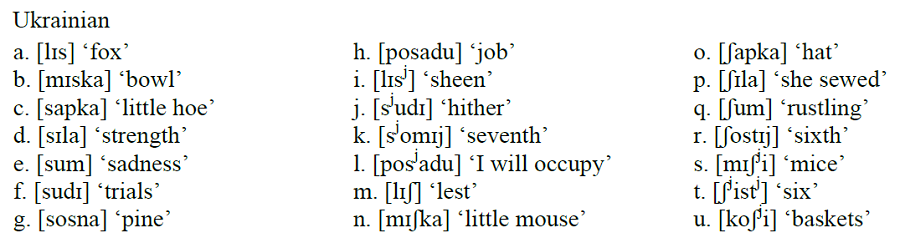
\includegraphics{../images/ukrainian.png}
\end{figure}

~\\
INSTRUCTOR NOTES: 


\newpage\textbf{\underline{\huge Phonological Relationships and Analysis / medium\\}}

~\\

{\large Question 1} - Source: Day 4 Discussion\\

Explain why we think that languages are not random in terms of their phonology.\\


~\\
INSTRUCTOR NOTES: 


~\\

{\large Question 2} - Source: Quiz 4, Question 5\\

What phonological relationships does this example show among the sounds [m], [n], and [ŋ], and why?\\

\begin{figure}[H]
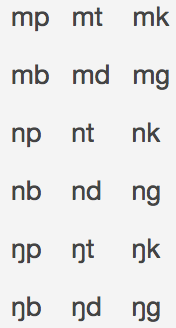
\includegraphics{../images/quiz4question5_a.png}
\end{figure}

~\\
INSTRUCTOR NOTES: contrast


~\\

{\large Question 3} - Source: Quiz 4, Question 5\\

What phonological relationships does this example show among the sounds [m], [n], and [ŋ], and why?\\

\begin{figure}[H]
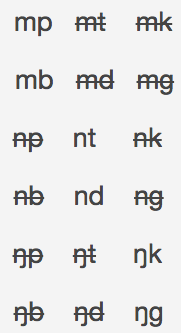
\includegraphics{../images/quiz4question5_b.png}
\end{figure}

~\\
INSTRUCTOR NOTES: allophony


~\\

{\large Question 4} - Source: Quiz 4, Question 5\\

What phonological relationships does this example show among the sounds [m], [n], and [ŋ], and why?\\

\begin{figure}[H]
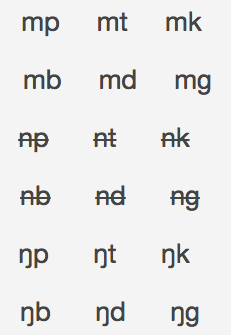
\includegraphics{../images/quiz4question5_c.png}
\end{figure}

~\\
INSTRUCTOR NOTES: contrast for [m] and [ŋ], but [n] doesn't occur


~\\

{\large Question 5} - Source: Quiz 4, Question 5\\

What phonological relationships does this example show among the sounds [m], [n], and [ŋ], and why?\\

\begin{figure}[H]
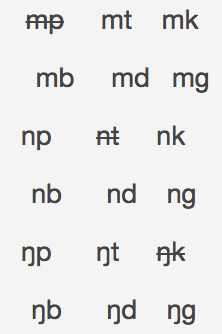
\includegraphics{../images/quiz4question5_d.png}
\end{figure}

~\\
INSTRUCTOR NOTES: contrast (with a few neutralizations)


~\\

{\large Question 6} - Source: Homework 2, Question 2\\

Why should the following two questions have the same answer?\\

\begin{itemize} \item Given the vowel system of Jita, how many bi-syllabic root types would you expect to find for nouns in the language? \item Assuming that the vowel inventory is the same in verbs as it is in nouns, how many bisyllabic root types would you expect to find for verbs in the language? \end{itemize}


~\\
INSTRUCTOR NOTES: 


~\\

{\large Question 7} - Source: Day 6 Handout, Question 5\\

Explain how you would determine the phonological relationship between these two sounds (given below) in this dataset.\\

{[pʰ]} and {[f]}

\begin{figure}[H]
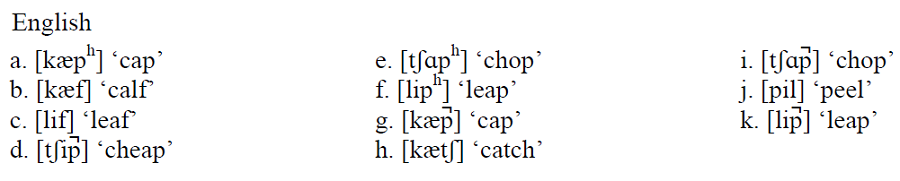
\includegraphics{../images/english_labials.png}
\end{figure}

~\\
INSTRUCTOR NOTES: contrastive; minimal pair


~\\

{\large Question 8} - Source: Day 6 Handout, Question 5\\

Explain how you would determine the phonological relationship between these two sounds (given below) in this dataset.\\

{[pʰ]} and {[p̚]}

\begin{figure}[H]
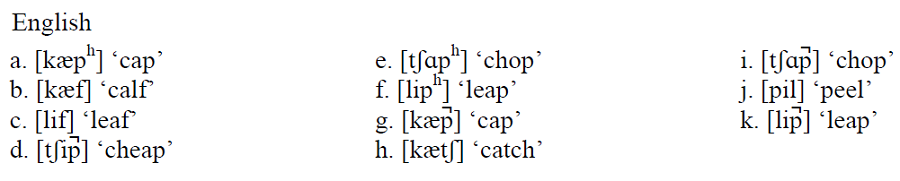
\includegraphics{../images/english_labials.png}
\end{figure}

~\\
INSTRUCTOR NOTES: free variation; pronunciation variants


~\\

{\large Question 9} - Source: Day 6 Handout, Question 6\\

Explain how you would determine the phonological relationship between these two sounds (given below) in this dataset.\\

{[l]} and {[ɾ]}

\begin{figure}[H]
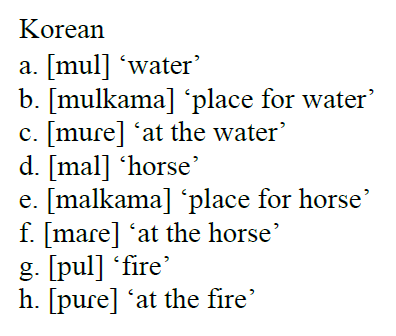
\includegraphics{../images/korean.png}
\end{figure}

~\\
INSTRUCTOR NOTES: allophonic; complementary distribution


~\\

{\large Question 10} - Source: Day 6 Handout, Question 7\\

Explain how you would determine the phonological relationship between these two sounds (given below) in this dataset.\\

{[m]} and {[n]}

\begin{figure}[H]
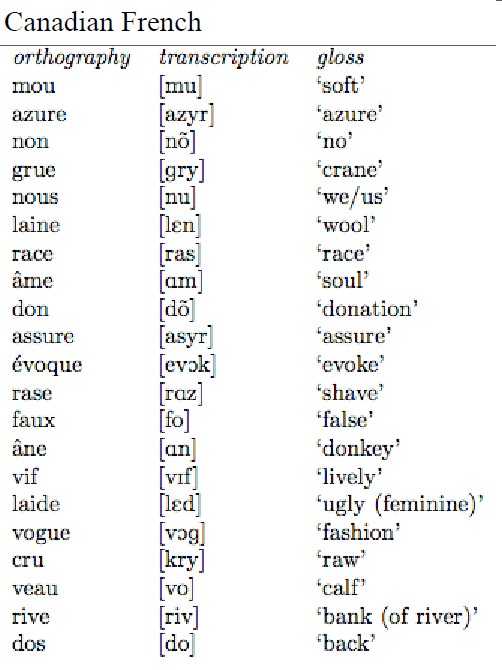
\includegraphics{../images/canadianfrench.png}
\end{figure}

~\\
INSTRUCTOR NOTES: contrastive; [mu] ‘soft’ vs. [nu] ‘we’


~\\

{\large Question 11} - Source: Day 6 Handout, Question 7\\

Explain how you would determine the phonological relationship between these two sounds (given below) in this dataset.\\

{[f]} and {[v]}

\begin{figure}[H]
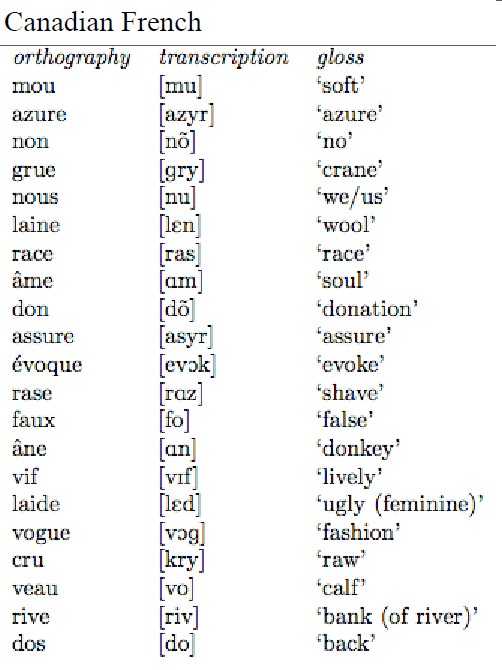
\includegraphics{../images/canadianfrench.png}
\end{figure}

~\\
INSTRUCTOR NOTES: contrastive; [fo] ‘false’ vs. [vo] ‘calf’


~\\

{\large Question 12} - Source: Day 6 Handout, Question 7\\

Explain how you would determine the phonological relationship between these two sounds (given below) in this dataset.\\

{[k]} and {[ɡ]}

\begin{figure}[H]
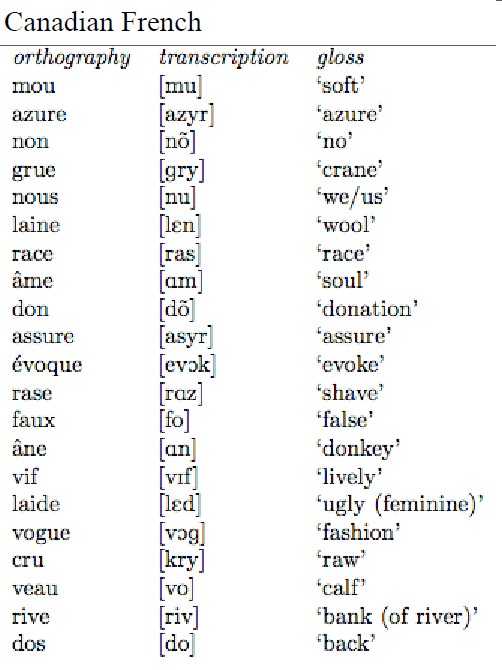
\includegraphics{../images/canadianfrench.png}
\end{figure}

~\\
INSTRUCTOR NOTES: contrastive; NEAR minimal pair; [evOk] ‘evoque’ vs. [vOg] ‘fashion’


~\\

{\large Question 13} - Source: Day 6 Handout, Question 7\\

Explain how you would determine the phonological relationship between these two sounds (given below) in this dataset.\\

{[d]} and {[n]}

\begin{figure}[H]
\includegraphics{../images/canadianfrench.png}
\end{figure}

~\\
INSTRUCTOR NOTES: contrastive; [do~] ‘donation’ vs. [no~] ‘no’


~\\

{\large Question 14} - Source: Day 6 Handout, Question 7\\

Explain how you would determine the phonological relationship between these two sounds (given below) in this dataset.\\

{[s]} and {[z]}

\begin{figure}[H]
\includegraphics{../images/canadianfrench.png}
\end{figure}

~\\
INSTRUCTOR NOTES: contrastive; [asyr] ‘assure’ vs. [azyr] ‘azure’


~\\

{\large Question 15} - Source: Day 6 Handout, Question 7\\

Explain how you would determine the phonological relationship between these two sounds (given below) in this dataset.\\

{[o]} and {[õ]}

\begin{figure}[H]
\includegraphics{../images/canadianfrench.png}
\end{figure}

~\\
INSTRUCTOR NOTES: contrastive; [do~] ‘donation’ vs. [do] ‘back’


~\\

{\large Question 16} - Source: Day 6 Handout, Question 9\\

Explain how you would determine the phonological relationship between these two sounds (given below) in this dataset.\\

{[l]} and {[ɫ]}

\begin{figure}[H]
\includegraphics{../images/english_laterals.png}
\end{figure}

~\\
INSTRUCTOR NOTES: [l] and [l̴] are allophonic in English. They are in complementary distribution, with [l] occurring before a vowel as in [lif] ‘leaf’ and [slɪm] ‘slim’ (and never after a vowel), and [l̴] occurring after a vowel, as in [fiɫ] ‘feel’ and [kɑɫd] ‘called’ (and never before a vowel).


~\\

{\large Question 17} - Source: Day 6 Handout, Question 5\\

Is the statement given below a good description of the distribution of sounds in this dataset? Why or why not?\\

The sounds {[pʰ]} and {[f]} are in complementary distribution. {[pʰ]} occurs after low vowels, as in {[kæpʰ]} ‘cap,’ while {[f]} occurs after high vowels, as in {[lif]} ‘leaf.’

\begin{figure}[H]
\includegraphics{../images/english_labials.png}
\end{figure}

~\\
INSTRUCTOR NOTES: no; the sounds are contrastive because there are minimal pairs, even though the example given isn't one


~\\

{\large Question 18} - Source: Day 6 Handout, Question 5\\

Is the statement given below a good description of the distribution of sounds in this dataset? Why or why not?\\

The sounds {[pʰ]} and {[p̚]} are in complementary distribution. {[pʰ]} occurs after front vowels, as in {[kæpʰ]} ‘cap,’ while {[p̚]} occurs after back vowels, as in {[tʃɑp̚]} ‘chop.’

\begin{figure}[H]
\includegraphics{../images/english_labials.png}
\end{figure}

~\\
INSTRUCTOR NOTES: no; the sounds are in free variation, because they can be variants of the same word, even though the example given doesn't show this


~\\

{\large Question 19} - Source: Day 6 Handout, Question 6\\

Is the statement given below a good description of the distribution of sounds in this dataset? Why or why not?\\

The sounds {[l]} and {[ɾ]} are in overlapping distribution. They can both occur after {[u]}, as in {[mul]} ‘water’ and {[muɾe]} ‘at the water.’ Thus, we know that these sounds are contrastive.

\begin{figure}[H]
\includegraphics{../images/korean.png}
\end{figure}

~\\
INSTRUCTOR NOTES: no; the sounds are allophonic, because the following environment is never the same


~\\

{\large Question 20} - Source: Day 6 Handout, Question 6\\

Is the statement given below a good description of the distribution of sounds in this dataset? Why or why not?\\

The sounds {[l]} and {[ɾ]} are in overlapping distribution, but just occur as pronunciation variants of the same morpheme, as in {[mul]} ‘water’ and {[muɾe]} ‘at the water.’ Thus, we know that these sounds are in free variation.

\begin{figure}[H]
\includegraphics{../images/korean.png}
\end{figure}

~\\
INSTRUCTOR NOTES: no; the sounds are allophonic, because the words are not actually identical -- these have different phonological contexts


~\\

{\large Question 21} - Source: Day 6 Handout, Question 9\\

Is the statement given below a good description of the distribution of sounds in this dataset? Why or why not?\\

The sounds {[l]} and {[ɫ]} are in complementary distribution. {[l]} occurs in onset position (before a vowel), but it becomes {[ɫ]} when it occurs in coda position (after a vowel).

\begin{figure}[H]
\includegraphics{../images/english_laterals.png}
\end{figure}

~\\
INSTRUCTOR NOTES: no; "becomes" is analytical, not descriptive


~\\

{\large Question 22} - Source: Day 6 Handout, Question 9\\

Is the statement given below a good description of the distribution of sounds in this dataset? Why or why not?\\

The sounds {[l]} and {[ɫ]} are in complementary distribution. {[ɫ]} occurs in coda position (after a vowel), but it turns into {[l]} when it occurs in onset position (before a vowel).

\begin{figure}[H]
\includegraphics{../images/english_laterals.png}
\end{figure}

~\\
INSTRUCTOR NOTES: no; "turns into" is analytical, not descriptive


~\\

{\large Question 23} - Source: Quiz 5, Question 2\\

State what kind of phonological relationship is shown between the sounds [o] and [a] and explain how you know.\\

\begin{figure}[H]
\includegraphics{../images/peng70ao_a.png}
\end{figure}

~\\
INSTRUCTOR NOTES: contrast (both occur after [i], [u], [a], and neither occurs after [o]); some neutralization in that [o] can't occur before [a] or [o], but [a] can


~\\

{\large Question 24} - Source: Quiz 5, Question 2\\

State what kind of phonological relationship is shown between the sounds [o] and [a] and explain how you know.\\

\begin{figure}[H]
\includegraphics{../images/peng70ao_b.png}
\end{figure}

~\\
INSTRUCTOR NOTES: contrast (both occur after [u], [o], [a] and before [o], [a]); neutralized after [i]


~\\

{\large Question 25} - Source: Quiz 5, Question 2\\

State what kind of phonological relationship is shown between the sounds [o] and [a] and explain how you know.\\

\begin{figure}[H]
\includegraphics{../images/peng70ao_c.png}
\end{figure}

~\\
INSTRUCTOR NOTES: allophony; [o] occurs only next to [o], and [a] occurs nect to any other vowel but not [o]


~\\

{\large Question 26} - Source: Quiz 5, Question 2\\

State what kind of phonological relationship is shown between the sounds [o] and [a] and explain how you know.\\

\begin{figure}[H]
\includegraphics{../images/peng70ao_d.png}
\end{figure}

~\\
INSTRUCTOR NOTES: contrast (both can occur everywhere -- no neutralization)


~\\

{\large Question 27} - Source: Day 7 Handout, Question 2\\

Explain whether the rule below would apply to the form shown, and if so, what the effect of the rule would be. Assume the vowel inventory [i], [ɪ], [e], [ɛ], [ɑ], [u], [ʊ], [o], [ɔ].\\

/isɪm/

{[high vowel]} →  {[unround, front]} / {[front vowel]} C$_0$ \_\_ 


~\\
INSTRUCTOR NOTES: applies; no effect


~\\

{\large Question 28} - Source: Day 7 Handout, Question 2\\

Explain whether the rule below would apply to the form shown, and if so, what the effect of the rule would be. Assume the vowel inventory [i], [ɪ], [e], [ɛ], [ɑ], [u], [ʊ], [o], [ɔ].\\

/ʊsɔm/

{[high vowel]} →  {[unround, front]} / {[front vowel]} C$_0$ \_\_ 


~\\
INSTRUCTOR NOTES: doesn't apply


~\\

{\large Question 29} - Source: Day 7 Handout, Question 2\\

Explain whether the rule below would apply to the form shown, and if so, what the effect of the rule would be. Assume the vowel inventory [i], [ɪ], [e], [ɛ], [ɑ], [u], [ʊ], [o], [ɔ].\\

/emɛs/

{[high vowel]} →  {[unround, front]} / {[front vowel]} C$_0$ \_\_ 


~\\
INSTRUCTOR NOTES: doesn't apply


~\\

{\large Question 30} - Source: Day 7 Handout, Question 2\\

Explain whether the rule below would apply to the form shown, and if so, what the effect of the rule would be. Assume the vowel inventory [i], [ɪ], [e], [ɛ], [ɑ], [u], [ʊ], [o], [ɔ].\\

/emus/

{[high vowel]} →  {[unround, front]} / {[front vowel]} C$_0$ \_\_ 


~\\
INSTRUCTOR NOTES: applies; [emis]


~\\

{\large Question 31} - Source: Day 7 Handout, Question 2\\

Explain whether the rule below would apply to the form shown, and if so, what the effect of the rule would be. Assume the vowel inventory [i], [ɪ], [e], [ɛ], [ɑ], [u], [ʊ], [o], [ɔ].\\

/emos/

{[high vowel]} →  {[unround, front]} / {[front vowel]} C$_0$ \_\_ 


~\\
INSTRUCTOR NOTES: doesn't apply


~\\

{\large Question 32} - Source: Day 7 Handout, Question 2\\

Explain whether the rule below would apply to the form shown, and if so, what the effect of the rule would be. Assume the vowel inventory [i], [ɪ], [e], [ɛ], [ɑ], [u], [ʊ], [o], [ɔ].\\

/imɑm/

{[high vowel]} →  {[unround, front]} / {[front vowel]} C$_0$ \_\_ 


~\\
INSTRUCTOR NOTES: doesn't apply


~\\

{\large Question 33} - Source: Day 7 Handout, Question 2\\

Explain whether the rule below would apply to the form shown, and if so, what the effect of the rule would be. Assume the vowel inventory [i], [ɪ], [e], [ɛ], [ɑ], [u], [ʊ], [o], [ɔ].\\

/isɪm/

{[non-low vowel]} →  {[lax]} / \_\_ C$_0$ {[lax vowel]}


~\\
INSTRUCTOR NOTES: applies; [ɪsɪm]


~\\

{\large Question 34} - Source: Day 7 Handout, Question 2\\

Explain whether the rule below would apply to the form shown, and if so, what the effect of the rule would be. Assume the vowel inventory [i], [ɪ], [e], [ɛ], [ɑ], [u], [ʊ], [o], [ɔ].\\

/ʊsɔm/

{[non-low vowel]} →  {[lax]} / \_\_ C$_0$ {[lax vowel]}


~\\
INSTRUCTOR NOTES: applies; no effect


~\\

{\large Question 35} - Source: Day 7 Handout, Question 2\\

Explain whether the rule below would apply to the form shown, and if so, what the effect of the rule would be. Assume the vowel inventory [i], [ɪ], [e], [ɛ], [ɑ], [u], [ʊ], [o], [ɔ].\\

/emɛs/

{[non-low vowel]} →  {[lax]} / \_\_ C$_0$ {[lax vowel]}


~\\
INSTRUCTOR NOTES: applies; [ɛmɛs]


~\\

{\large Question 36} - Source: Day 7 Handout, Question 2\\

Explain whether the rule below would apply to the form shown, and if so, what the effect of the rule would be. Assume the vowel inventory [i], [ɪ], [e], [ɛ], [ɑ], [u], [ʊ], [o], [ɔ].\\

/emus/

{[non-low vowel]} →  {[lax]} / \_\_ C$_0$ {[lax vowel]}


~\\
INSTRUCTOR NOTES: doesn't apply


~\\

{\large Question 37} - Source: Day 7 Handout, Question 2\\

Explain whether the rule below would apply to the form shown, and if so, what the effect of the rule would be. Assume the vowel inventory [i], [ɪ], [e], [ɛ], [ɑ], [u], [ʊ], [o], [ɔ].\\

/emos/

{[non-low vowel]} →  {[lax]} / \_\_ C$_0$ {[lax vowel]}


~\\
INSTRUCTOR NOTES: doesn't apply


~\\

{\large Question 38} - Source: Day 7 Handout, Question 2\\

Explain whether the rule below would apply to the form shown, and if so, what the effect of the rule would be. Assume the vowel inventory [i], [ɪ], [e], [ɛ], [ɑ], [u], [ʊ], [o], [ɔ].\\

/imɑm/

{[non-low vowel]} →  {[lax]} / \_\_ C$_0$ {[lax vowel]}


~\\
INSTRUCTOR NOTES: doesn't apply (unless [ɑ] treated as lax)


~\\

{\large Question 39} - Source: Day 7 Handout, Question 7\\

Explain how you would choose the underlying representation of the phoneme with allophones [s] and [ʃ].\\

\begin{figure}[H]
\includegraphics{../images/japanese.png}
\end{figure}

~\\
INSTRUCTOR NOTES: We would probably pick the alveolar version /s/ to be the underlying representation, because it occurs in a wider set of contexts. That way, we can write a single rule to derive the more limited distribution of the palatal, and not need rules to explain any of alveolar occurrences.


~\\

{\large Question 40} - Source: Day 7 Handout, Question 7\\

Explain how you would choose the underlying representation of the phoneme with allophones [z] and [dʒ].\\

\begin{figure}[H]
\includegraphics{../images/japanese.png}
\end{figure}

~\\
INSTRUCTOR NOTES: We would probably pick the alveolar version /z/ to be the underlying representation, because it occurs in a wider set of contexts. That way, we can write a single rule to derive the more limited distribution of the palatal, and not need rules to explain any of alveolar occurrences.


~\\

{\large Question 41} - Source: Day 7 Handout, Question 8\\

Explain how you would choose the underlying representation for the phoneme with allophones [ʊ] and [ɯ].\\

\begin{figure}[H]
\includegraphics{../images/tamil.png}
\end{figure}

~\\
INSTRUCTOR NOTES: The phoneme category should be /ʊ/, because it occurs in the wider range of situations – especially when there is no preceding vowel that would condition whether it should be rounded or not. That is, it seems to the be “default” vowel.


\newpage\textbf{\underline{\huge Phonological Relationships and Analysis / very hard\\}}

~\\

{\large Question 1} - Source: Day 6 Handout, Question 11\\

What do the two signs below tell you about the phonological status of \underline{handshape} in ASL, and why?\\

\begin{figure}[H]
\includegraphics{../images/asl_apple.png}
\caption{APPLE}
\end{figure}
\begin{figure}[H]
\includegraphics{../images/asl_candy.png}
\caption{CANDY}
\end{figure}

~\\
INSTRUCTOR NOTES: shows contrast because movement and location are same


~\\

{\large Question 2} - Source: Day 6 Handout, Question 11\\

What do the two signs below tell you about the phonological status of \underline{handshape} in ASL, and why?\\

\begin{figure}[H]
\includegraphics{../images/asl_stay.png}
\caption{STAY}
\end{figure}
\begin{figure}[H]
\includegraphics{../images/asl_awkward.png}
\caption{AWKWARD}
\end{figure}

~\\
INSTRUCTOR NOTES: nothing, because both handshape and movement are different


~\\

{\large Question 3} - Source: Day 6 Handout, Question 11\\

What do the two signs below tell you about the phonological status of \underline{handshape} in ASL, and why?\\

\begin{figure}[H]
\includegraphics{../images/asl_apple.png}
\caption{APPLE}
\end{figure}
\begin{figure}[H]
\includegraphics{../images/asl_now.png}
\caption{NOW}
\end{figure}

~\\
INSTRUCTOR NOTES: nothing, because handshape and location and movement are all also different


~\\

{\large Question 4} - Source: Day 7 Handout, Question 9\\

What is the basic analysis of vowel length in this dataset, and what are the key pieces of evidence?\\

\begin{figure}[H]
\includegraphics{../images/malayalam.png}
\end{figure}

~\\
INSTRUCTOR NOTES: Short and long vowels appear to be contrastive (phonemic) in Malayalam, as evidenced by minimal pairs that differ only in terms of their vowel length, such as [koʈːa] ‘basket’ vs. [koːʈːa] ‘castle’ or [keʈːu] ‘burnt out’ vs. [keːʈːu] ‘heard.’


~\\

{\large Question 5} - Source: Day 7 Handout, Question 11\\

What is the basic analysis of voiceless stops in this dataset, and what are the key pieces of evidence?\\

\begin{figure}[H]
\includegraphics{../images/english11.png}
\end{figure}

~\\
INSTRUCTOR NOTES: Plain and aspirated voiceless stops are in complementary distribution in English. Plain stops occur always and only after [s], as in [speɪs] ‘space,’ while aspirated stops never occur in this context. Meanwhile, aspirated stops occur word-initially (e.g., [phitʃ] ‘peach’) and between vowels (e.g., [əphɑɹt] ‘apart’). Because the two are in complementary distribution, we can always predict which one occurs in any given environment, and so we conclude that they are allophonic, i.e., allophones of the same phoneme category. 


~\\

{\large Question 6} - Source: Day 7 Handout, Question 12\\

What is the basic analysis of oral and nasal vowels in this dataset, and what are the key pieces of evidence?\\

\begin{figure}[H]
\includegraphics{../images/english12.png}
\end{figure}

~\\
INSTRUCTOR NOTES: The pairs of sounds [i] and [ĩ], and [u] and [ũ], are each allophonic and therefore allophones of the same phoneme in English (though the two pairs represent two contrastive phonemes in English). The sounds [i] and [ĩ] are in complementary distribution in English, with [ĩ] occurring before the sounds [m] and [n], (e.g., [ɡlĩm] ‘gleam’ and [klĩn] ‘clean’) and [i] occurring elsewhere (e.g., [lip] ‘leap’). Similarly, the sounds [u] and [ũ] are also in complementary distribution, with exactly the same conditioning environments: [ũ] occurs before [m] and [n] (e.g., [dũm] ‘doom’ and [dũn] ‘dune’), and [u] occurs elsewhere (e.g. [but] ‘boot’). Thus, within each pair, we treat the vowels as allophonic. 


\newpage\textbf{\underline{\huge Phonological Relationships and Analysis / easy\\}}

~\\

{\large Question 1} - Source: Quiz 5, Question 10\\

Explain why the statement below either is or is not a good analysis of the data.\\

Because {[r]} and {[r̥]} are contrastive in English, we cannot write a rule to account for their distribution.

\begin{figure}[H]
\includegraphics{../images/peng71_englishr.png}
\end{figure}

~\\
INSTRUCTOR NOTES: not a good analysis because the two sounds are in complementary distribution


~\\

{\large Question 2} - Source: Quiz 5, Question 10\\

Explain why the statement below either is or is not a good analysis of the data.\\

We should posit /r/ as the underlying form, and have a rule that devoices it when it occurs after voiceless segments. This analysis is best because it requires only one rule with a single environment to account for all the occurrences of both {[r]} and {[r̥]}; the plain {[r]} sounds result from non-application of the rule.

\begin{figure}[H]
\includegraphics{../images/peng71_englishr.png}
\end{figure}

~\\
INSTRUCTOR NOTES: a good analysis


~\\

{\large Question 3} - Source: Quiz 5, Question 10\\

Explain why the statement below either is or is not a good analysis of the data.\\

We should posit /r̥/ as the underlying form, and have a rule that voices it when it occurs after voiced segments or word-initially. This analysis is best because it puts the more unusual sound, the voiceless {[r̥]}, into the underlying representation, which has to be memorized anyway.

\begin{figure}[H]
\includegraphics{../images/peng71_englishr.png}
\end{figure}

~\\
INSTRUCTOR NOTES: not a good analysis, because we want the UR to occur in the MOST environments, not the FEWEST (makes the rule simpler)


~\\

{\large Question 4} - Source: Quiz 5, Question 10\\

Explain why the statement below either is or is not a good analysis of the data.\\

Because {[r]} and {[r̥]} are in free variation in English, we cannot write a rule to account for their distribution.

\begin{figure}[H]
\includegraphics{../images/peng71_englishr.png}
\end{figure}

~\\
INSTRUCTOR NOTES: not a good analysis, because the sounds are in complementary distribution


~\\

{\large Question 5} - Source: Day 7 Handout, Question 1\\

Explain what the rule below does and suggest a name for it, explaining why that would be a good name.\\

/n/ → {[m]} / \_\_ \{{[p]}, {[b]}\}


~\\
INSTRUCTOR NOTES: 


~\\

{\large Question 6} - Source: Day 7 Handout, Question 1\\

Explain what the rule below does and suggest a name for it, explaining why that would be a good name.\\

/n/ → {[ŋ]} / \_\_ {[velar]}


~\\
INSTRUCTOR NOTES: 


~\\

{\large Question 7} - Source: Day 7 Handout, Question 1\\

Explain what the rule below does and suggest a name for it, explaining why that would be a good name.\\

{[nasal]} → {[αPlace]} / \_\_ {[αPlace]}


~\\
INSTRUCTOR NOTES: 


~\\

{\large Question 8} - Source: Day 7 Handout, Question 1\\

Explain what the rule below does and suggest a name for it, explaining why that would be a good name.\\

{[vowel]} → {[nasal]} / {[nasal]} \_\_


~\\
INSTRUCTOR NOTES: 


~\\

{\large Question 9} - Source: Day 7 Handout, Question 1\\

Explain what the rule below does and suggest a name for it, explaining why that would be a good name.\\

{[high vowel]} →  {[unround, front]} / {[front vowel]} C$_0$ \_\_


~\\
INSTRUCTOR NOTES: 


~\\

{\large Question 10} - Source: Day 7 Handout, Question 1\\

Explain what the rule below does and suggest a name for it, explaining why that would be a good name.\\

{[non-low vowel]} →  {[lax]} / \_\_ C$_0$ {[lax vowel]}


~\\
INSTRUCTOR NOTES: 


\newpage\end{document}

